\documentclass[submission,copyright,creativecommons]{eptcs}
\providecommand{\event}{TLLA 2022} % Name of the event you are submitting to
\usepackage{breakurl}             % Not needed if you use pdflatex only.
\usepackage{underscore}           % Only needed if you use pdflatex.

%myPackages
\usepackage[T1]{fontenc} 
\usepackage[utf8]{inputenc} 
\usepackage{lmodern} 
\usepackage[english]{babel} 
\usepackage{amssymb}  
\usepackage{stmaryrd} 
\usepackage{amsthm}
\usepackage{amsmath}
\usepackage{comment}
\usepackage{ebproof}
\usepackage{tkz-graph}
\usepackage{tikz}
\usepackage{tikz-cd}
\usetikzlibrary {positioning}
\usepackage{cmll}
\usepackage{mathrsfs}
\usepackage{marvosym}
\usepackage{cancel}
\usepackage{pst-solides3d}
\usepackage{MnSymbol}
\usetikzlibrary{matrix,arrows,decorations.pathmorphing,calc}
\usepackage[top=1in, bottom=1.25in, left=1in, right=1in]{geometry}

\setlength{\parindent}{0.7em}
\setlength{\parskip}{1.3em}

%\bibliographystyle{alpha}

\newtheorem{theorem}{Theorem}[section]
\newtheorem{Lemma}[theorem]{Lemma}
\newtheorem{Proposition}[theorem]{Proposition}
\newtheorem{Corollary}[theorem]{Corollary}
\newtheorem{Definition}[theorem]{Definition}
\newtheorem{Example}[theorem]{Example}
\newtheorem{Remark}[theorem]{Remark}
\newtheorem{Notation}[theorem]{Notation}
\newtheorem{Terminology}[theorem]{Terminology}

\newcommand\eg{\textit{e.g.\ }}
\newcommand\etc{\textit{etc}}

\newtheorem{lemma}{Lemma}
\newtheorem{corollary}{Corollary}
\newtheorem{claim}{Claim}
\newtheorem{proposition}{Proposition}
\newtheorem{remark}{Remark}
\newtheorem{notation}{Notation}
\newtheorem{definition}{Definition}
\newtheorem{example}{Example}
\newtheorem{assumption}{Assumption}

\newcommand{\iu}{û}
\newcommand{\e}{ê}
\newcommand{\A}{â}
\newcommand{\Xplus}{X^{+}}
\newcommand{\forces}{\ \digamma}
\newcommand{\cons}{\textbf{.}}
\newcommand{\brabra}[1]{\llbracket #1 \rrbracket}
\newcommand{\test}[1]{\Vert #1 \Vert}
\newcommand{\str}[1]{\vert #1 \vert}
\newcommand{\sub}[3]{#1\{#2/#3\}}
\newcommand{\oppose}[3]{#1 \not\varepsilon #2^{+}(#3)}
\newcommand{\prog}[1]{\texttt{\small{\textbf{#1}}}}
\newcommand{\callcc}{\prog{callcc}}
\newcommand{\parts}{\mathcal{P}}
\newcommand{\fparts}{\parts_{f}}
\newcommand{\N}{\mathbb{N}}
\newcommand{\R}{\mathbb{R}}
\newcommand{\Var}{\mathrm{Var}}
\newcommand{\rbeta}{\rightarrow_{\beta}}
\newcommand{\infer}[2]{\dfrac{#2}{#1}}
\newcommand{\interpret}[1]{\llbracket #1\rrbracket}
\newcommand{\Env}[1]{\mathrm{Env}_{#1}}
\newcommand{\restr}[2]{#1_{\big|_{#2}}}
\newcommand{\linc}{c^\bullet}

\usepackage{setspace}

% General Symbols
\newcommand{\nat}{\mathbb{N}} % natural numbers
\newcommand\seq\vec % sequence
\newcommand{\st}{s.t.\ } % Such that
\newcommand{\set}[1]{\{#1\}}
\newcommand{\bnfeq}{::=}
\newcommand\pow[1]{\mathscr{P}(#1)}  % powerset
\newcommand{\void}{\varnothing} % empty set
\newcommand{\fmsets}[1]{\mathcal{M}_f(#1)} % set of finite multisets on #1
\newcommand{\emptymset}{1} % empty multyset
\newcommand\bpf{\begin{proof}}
\newcommand\epf{\end{proof}}
\newcommand{\cT}{\mathcal{T}}
\newcommand{\cH}{\mathcal{H}}
\newcommand\cX{\mathcal{X}}
\newcommand{\finsub}{\subseteq
\newcommand{\cL}{\mathcal{L}}_\mathrm{f}}
% Lambda calculus
\newcommand{\lam}{\ensuremath{\lambda}}
\newcommand{\lamu}{\lambda\mu}
\newcommand{\Lam}{\ensuremath{\Lambda}}
\newcommand{\Lamo}{\Lambda^o}
\newcommand{\lamb}{\ensuremath{\lambda\bot}}
\newcommand{\subst}[2]{\{#2/#1\}} % substitution
\newcommand{\cB}{\mathcal{B}} % B of Bohm tree theory
\newcommand{\msto}[1][]{\twoheadrightarrow_{#1}} % multistep reduction
\newcommand{\holes}[1]{\langle #1\rangle} % context holes
\newcommand{\LamContext}[1]{\Lam\holes{#1}} % Lam<\xi>
\newcommand{\FV}[1]{\mathrm{FV}(#1)} % free variables
\newcommand{\BT}[1]{\mathrm{BT}(#1)} % BT(M)
\newcommand{\App}[1]{\mathcal{A}(#1)} % Approximants(M)
\newcommand{\Appr}{\mathcal{A}pp} % Set of all the approximants
\newcommand{\BTle}{\le_\bot} % <=_\Bot
\newcommand{\BTge}{\ge_\bot}
\newcommand{\comb}[1]{\mathsf{#1}}
\newcommand{\bI}{\comb{I}}
\newcommand{\rel}[1]{\mathtt{#1}}
\newcommand{\Om}{\comb{\Omega}}
\newcommand{\blam}{\boldsymbol{\lambda}}
\newcommand{\sqle}{\sqsubseteq}
\newcommand{\TM}[2][]{\mathcal{M}_{#2}^{#1}}
\newcommand{\fresh}{\mathrel{\#}}
\newcommand{\namedapp}[3]{(#1)_#2 #3}
% Resource calculus
\newcommand{\bag}[1]{{[}#1{]}}
\newcommand{\sums}[1]{\Bool\langle #1 \rangle} % 2<Lam^r>
\newcommand{\Bool}{\mathsf{2}} % ring 0,1
\newcommand{\Lamr}{\Lambda^r} % set of resource terms
\newcommand{\Lamb}{\Lambda^b} % set of bags
\newcommand{\lsubst}[2]{\langle [#2]/#1\rangle} % linear substitution
\newcommand{\Sum}[1]{\mathbb{#1}} % Sum of terms
\newcommand{\Te}[1]{\mathcal{T}(#1)} % (support of) Taylor expansion
\newcommand{\NF}[2][]{\mathrm{NF}_{#1}(#2)} % Normal form
\newcommand{\ResContext}[1]{\Lamr\holes{#1}} % Lam^r<\xi>
\newcommand{\BagResContext}[1]{\Lamb\holes{#1}} % Lam^b<\xi>
\newcommand{\NFTeq}{=_\tau} % "=_\tau", meaning NF(T(M)) = NF(T(M))
\newcommand{\size}[1]{\mid#1\mid} % size of a resource term
\newcommand{\nf}[2][]{\mathrm{nf}_{#1}(#2)}
\newcommand{\NFT}[1]{\mathrm{NF}\mathcal{T}(#1)}
\newcommand{\lin}[1]{#1^\circ}
\newcommand{\nak}[1]{|#1|}
\newcommand{\tor}{\to_r}
\newcommand{\redto}[1][]{\to_{#1}}
\newcommand{\emptybag}{1}
\newcommand{\forg}[1]{\lfloor #1\rfloor}
\newcommand\hole[1]{\llparenthesis\hspace{1pt} #1\hspace{1pt} \rrparenthesis} %context hole
\newcommand\linsub[2]{\langle #2 / #1 \rangle} %t<b/x> (lin sub without writing "[]" fo the bags)
\newcommand\lnamedapp[3]{\langle #1 \rangle_{#2} #3}
\newcommand\bigstep{\rightrightarrows}

%MACROS GIULIO
%!TEX root = ../BarbaM.tex
%%%%%% Lambda
\newcommand{\bnf}{::=}
\newcommand{\Appof}[1]{\mathcal{A}(#1)}
\newcommand{\approf}[1]{P_{#1}}
\newcommand{\bool}{\mathsf{2}}
\newcommand\Mfin[1]{\mathcal{M}_\mathrm{f}(#1)}
\newcommand{\cJ}{\mathcal{J}}
\newcommand{\cI}{\mathcal{I}}
\newcommand{\PLL}{\textsf{PLL}}
\newcommand\dg[2]{\mathrm{deg}_{#1}(#2)}
\newcommand{\comp}[1]{#1\!\!\uparrow}

\newcommand{\Pfinstar}[1]{\mathscr{P}_\mathrm{fin}^*(#1)}
\newcommand{\web}[1]{\lvert #1\lvert}
\newcommand{\homology}[2]{\mathcal{H}_{#1}(#2)}
\newcommand{\cs}[1]{\mathrm{cs}(#1)}
\newcommand{\simplices}[1]{\mathcal{S}#1}
\newcommand{\orsimpl}[2]{\overrightarrow{\mathcal S_{#1}} #2}
\newcommand{\barIexp}[2]{\mathscr{I}^{#1}\!#2}
\newcommand{\barI}[1]{\mathscr{I}\!#1}
\newcommand{\barsubd}[1]{\mathbf{bs}(#1)}

\newcommand{\lolli}{\multimap}
\newcommand{\cutelim}{\rightsquigarrow}

\newcommand{\minimum}[2]{\emph{min}\{#1,#2\}}

\newcommand{\alarm}[1]{\color{red}#1\color{black}}

\newcommand{\qRel}[1]{\mathrm{Rel_{#1}}}

\newcommand{\eps}{\epsilon}

\newcommand{\norm}[1]{\lVert #1 \lVert}
\newcommand{\supnorm}[1]{\lVert #1 \lVert_\infty}
\newcommand{\absv}[1]{\mid #1\mid}

\title{Denotational semantics driven simplicial homology?}
\author{Davide Barbarossa\thanks{Thanks to Thomas Ehrhard who contributed to this work. Thanks also to Giulio Manzonetto and Lorenzo Tortora de Falco for instructive discussions.}
%\institute{Università di Bologna\\ Bologna, Italia}
\institute{Dipartimento di Informatica: Scienza ed Ingegneria\\
Università di Bologna%\\ Bologna, Italia\thanks{A fine university.}
\\
Bologna, Italia}
\email{davide.barbarossa@unibo.it}
%\and
%Co Author \qquad\qquad Yet S. Else
%\institute{Stanford Univeristy\\
%California, USA}
%\email{\quad is@gmail.com \quad\qquad somebody@else.org}
}
\def\titlerunning{Den.\ sem.\ and homology}
\def\authorrunning{Davide Barbarossa}
\begin{document}

%\maketitle

%\begin{abstract}
%\end{abstract}

\begin{Definition}
Let $R$ be a semiring.
The category $\mathrm{Rel}_R$ has sets as objects, and the homset $\mathrm{Rel}_R(X,Y)$ is the set $R^{X\times Y}$ of matrices with rows indexed by $X$, columns indexed by $Y$ and coefficients in $R$.
The identity $id_X$ is the usual diagonal matrix $id_{a,b}:=\delta_{a,b}$ ($\delta$ is the Kronecker symbol), and the composition of $t:Y\times Z\to R$ with $s:X\times Y\to R$ is the matrix $ts:X\times Z\to R$ given by $(ts)_{a,c}:=\sum\limits_{b\in Y} t_{b,c}s_{a,b}$.
We suppose for the moment that all the desired infinite series converge in $R$.
\end{Definition}

Our composition formula is slightly unconventional.
This is because, usually, a matrix $t$ with raws on $X$ and columns on $Y$ is seen as a function from $R^Y$ to $R^X$ ($R$ being here any set of coefficients);
however, we are using the opposite convention, which corresponds to taking the transpose.
In this way, the matrix $t$ applies to a vector $x\in R^X$ giving rise to a vector $tx\in R^Y$ (instead of the converse), and the formula takes the (slightly unconventional) form $(tx)_{b} := \sum\limits_{a\in X} t_{a,b}x_{a}$.
We use this convention because it simplifies notations, as it allows us to see matrices $t\in\mathrm{Rel}_R(X,Y)$ as functions $\hat{t}:R^X\to R^Y$.

\begin{Remark}
It is straightforward to see that each $R^X$ is a $R$-\emph{module} w.r.t.\ pointwise scalar multiplication and pointwise addition.
\alarm{If the desired infinite series behave well in $R$, then the functions $\hat{t}$ are all and only the linear ones, as in the finite case.}
\end{Remark}

Given $a\in X$, let us denote by $e_a\in Q^X$ the ``canonical base vector'' whose coordinates are $(e_a)_{a}:=1$ and $(e_a)_{a'}:=0$ if $a\neq a'$.

Let us set $\overline{\R}_{\geq 0}:=\R_{\geq 0}\cup\set{+\infty}$.

\begin{Terminology}
Consider the complete lattice $(\overline{\R}_{\geq 0},\geq)$, with joins $\bigvee A$ given by $\inf A$, and meets $\bigwedge A$ by $\sup A$.
Remark that we set $\inf \emptyset := +\infty$.
It becomes a semiring if we endow it with $\inf$ as addition and $+$ as multiplication\footnote{The neutral element for addition being $+\infty$ and the one for multiplication $0$.}.
It is called the \emph{non-negative (min-plus-)tropical (commutative and idempotent) semiring}.
Moreover, it is a (unital, commutative, idempotent) quantale with multiplication the one of its semiring structure (that is, $+$).
It is also a continuous semiring.
Let us call it $Q$.
\end{Terminology}

\begin{Remark}
The $Q$-module structure of $Q^X$ is given by scalar multiplication $(r,x)\in Q\times Q^X\to r+x\in Q^X$ and addition $(x,y)\in Q\times Q^X\to \minimum{x}{y}\in Q^X$.
\alarm{If $t\in\mathrm{Rel}_Q(X,Y)$, than the function $\hat{t}$ is \emph{linear}}.
\end{Remark}

\begin{Definition}
Let us call $\mathrm{Trop}$ the co-Kleisli category $(\mathrm{Rel}_Q)_!$ of $\mathrm{Rel}_Q$ w.r.t.\ the usual multiset comonad $!$.
That is, objects are sets and morphisms from $X$ to $Y$ are matrices $F:\fmsets{X}\times Y\to Q$, seen as maps $\hat{F}:Q^{\fmsets{X}}\to Q^Y$.
Moreover, the identity on $X$ is the function $id:\fmsets{X}\times X\to X$ s.t.\ $id_{[x],x}=0$ and $id_{\mu,x}=+\infty$ if $\mu\neq [x]$, and the composition $GF:\fmsets{X}\times Z\to Q$ of $G:\fmsets{Y}\times Z\to R$ with $F:\fmsets{X}\times Y\to R$ takes the form:
\[
 (GF)_{\mu,c} = \inf\limits_{\rho\in\fmsets{Y}} \left\{G_{\rho,c}+\sum\limits_{b\in Y} \rho_b F_{\mu,b}\right\}.
\]
The induced map $\hat{F}:Q^{\fmsets{X}}\to Q^Y$ by $F\in\mathrm{Trop}(X,Y)$ is given by:
\[
 \hat{F}(x)_b = \inf\limits_{\mu\in\fmsets{X}} \left\{F_{\mu,b}+\mu\cdot x\right\}
\]
where $\mu\cdot x := \sum\limits_{a\in X} \mu_a x_a \in Q$.
We call \emph{tropical analytical} the functions of the shape $\hat{F}$.
\end{Definition}

\begin{Remark}
Since $Q$ is a continuous semiring, [Weighted relational models] assures us that $\mathrm{Rel}_Q$ is:

- linear and continuous category

- $*$-autonomous with biproducts and bilinear and continuous tensor and monoidal currying

- Lafont category.

Furthermore, the same paper tells us that $(\mathrm{Rel}_Q)_!$ is a post-linear and continuous $Q$-CCC.
\end{Remark}

\begin{Example}
The terminal object of $\mathrm{Trop}$ is $1:=\set{*}$.
Using the trivial bijection $\fmsets{\set{*}}= \N$, the morphisms $F\in\mathrm{Trop}(1,1)$ are \emph{exactly} the functions $F:\N\to Q$, and the induced tropical analytical map $\hat F: Q=Q^{\set{*}}\to Q^{\set{*}}=Q$ has shape $\hat{F}(x)=\inf\limits_{n\N}\set{F(n)+nx}$.
A particular case is the one of tropical polynomials on $Q$, which coincide with the tropical analytical functions from $Q$ to itself for which the $\inf$ is always a $\min$.
In particular, all affine functions $\hat F(x)=r+mx$ \emph{with $m\in\N$}, $r\in Q$ from $Q$ to itself (and thus also all affine functions from $\R$ to itself), are of this shape: is suffices to take $F(n):=r$ if $n=m$ and $F(n)=+\infty$ otherwise.
\end{Example}

\begin{Remark}
We can endow $Q^X$ with two (potentially $+\infty$) metrics:
\[d^{\infty}(x,y):=\sup\limits_{a\in X}|x_a-y_a|\]
\[d^1(x,y):=\sum\limits_{a\in X}|x_a-y_a|. \alarm{(Forse \ questa \ la \ si \ dovrebbe \ prendere \ tropicale, \ ovvero \ inf_a ?)}\]
\end{Remark}

Remember the following easy property of infs and sequences.

\begin{Lemma}
If $\mid a_n-b_n\mid \,\leq K$ for all $n \in\N$, then $\mid \inf\limits_n a_n-\inf\limits_n b_n\mid \,\leq K$.
\end{Lemma}
\begin{proof}
We have $\mid \inf\limits_n b_n - \inf\limits_n a_n\mid \leq \mid \inf\limits_n b_n - b_{m}\mid + \mid b_{m} - a_m\mid + \mid a_m - \inf\limits_n a_n\mid\leq \mid \inf\limits_n b_n - b_{m}\mid + K + \mid a_m - \inf\limits_n a_n\mid$  for all $m\in\N$, so $\mid \inf\limits_n b_n - \inf\limits_n a_n\mid \leq \inf\limits_m \set{\mid \inf\limits_n b_n - b_{m}\mid + K + \mid a_m - \inf\limits_n a_n\mid} = K$.
\end{proof}

Let us call $\widetilde{F}_{\mu,b}(x):=F_{\mu,b}+\mu\cdot x$, so that $\hat{F}(x)_b = \inf\limits_{\mu\in\fmsets{X}} \widetilde{F}_{\mu,b}(x)$.

\begin{Remark}
Let $\hat F, \hat G : Q^X\to Q^Y$ tropical analytical, whose associated matrices are $F,G$ respectively.
We have:
\[
 d^{\infty}(\hat F(x),\hat{G}(x)) \leq  d^{\infty}(F,G)
\]
for all $x\in Q^X$.

Indeed, we have:
$|\widetilde{F}_{\mu,b}(x)-\widetilde{G}_{\mu,b}(x)|=|F_{\mu,b}-G_{\mu,b}|\leq d^{\infty}(F,G)$, so by the previous Lemma $|\hat F(x)_b-\hat{G}(x)_b|\leq d^{\infty}(F,G)$ and thus the desired result.
\end{Remark}

\begin{Remark}
The functions $\widetilde{F}_{\mu,b}$ are $\#\mu$-Lipschitz in $Q^X$ (w.r.t.\ both metrics).
Indeed we have the following straightforward inequalities:
\[
 |\widetilde{F}_{\mu,b}(x)-\widetilde{F}_{\mu,b}(y)| =
 | \mu\cdot (x-y) | \leq
 \mu\cdot| x-y | =
 \sum\limits_{a\in X} \mu_a | x_a - y_a | \leq
 d(x,y)\sum\limits_{a\in X} \mu_a = 
 d(x,y)\#\mu.
\]
\end{Remark}

\begin{Remark}
The functions $\widetilde{F}_{\mu,b}$ are always non-decreasing, in the sense that $\widetilde{F}_{\mu,b}(x)\leq \widetilde{F}_{\mu,b}(x+y)$.
This is clear because everything takes place in non-negative real numbers, so $\mu\cdot x\leq \mu\cdot (x+y)$.
Therefore, also $\hat{F}$ is non-decreasing (in the same sense: for all $b\in Y$, we have $\hat F (x)_b\leq \hat F (x+y)_b$).
\end{Remark}

\begin{Remark}
Fix $\epsilon>0$.
Then there is $\mu^\epsilon\in\fmsets{X}$ s.t.\ $|\hat{F}(x)_b-\widetilde{F}_{\mu^\epsilon,b}(x)|\leq\epsilon$ (this is by definition of $\inf$).
Furthermore, if $\hat F(x)_b < +\infty$ then $\sum\limits_{a\in X} \mu^\epsilon_a x_a=\mu^\epsilon\cdot x < +\infty$.
This means that $\mu^\epsilon_a x_a<+\infty$ for all $a\in X$.

Actually, for all $a\in X$, there must exist $K_a\in\R$ s.t.\ $\mu^\epsilon_a x_a \leq K_a$ for all $0<\epsilon<1$ \alarm{(limitare eps serve altrimenti l'argomento sotto non funziona!)}.
In fact, otherwise, there is an $a\in X$ s.t.\ for all $K_a$ there is $0<\epsilon<1$ s.t.\ $\widetilde{F}_{\mu^\epsilon,b}(x)\geq \mu^\epsilon_a x_a> K_a$.
But, taking $K_a$ large enough, we obtain a contradiction with he fact that, by definition of $\mu^\epsilon$, we must have $|\hat{F}(x)_b-\widetilde{F}_{\mu^\epsilon,b}(x)|\leq\epsilon<1$.

Therefore, for all $a\in X$ s.t.\ $x_a\neq 0$, there must still exist $L_a\in\R$ s.t.\ $\mu^\epsilon_a \leq L_a$ for all $0<\epsilon<1$.
\end{Remark}

\begin{Remark}
Let $q\in Q$. For all $0<\epsilon<1$, we have:
\[
 |\widetilde{F}_{\mu^\epsilon,b}(x)-\widetilde{F}_{\mu^\epsilon,b}(x+ qe_a)| =
 | \mu^\epsilon\cdot (-qe_a) |=
 q\mu^\epsilon_a\]
and, if $x_a\neq 0$, the inequality continues as $\leq qL_a$.
\end{Remark}

Putting all this together we get:

\begin{Proposition}
Let $\hat F$ tropical analytical.
Fix $x\in Q^X$ and let $a\in X$ s.t.\ $x_a\neq 0$.
For all $0<\epsilon<1$ we have:
\[
 |\hat{F}(x)_b - \hat{F}(x+ \epsilon e_a)_b| \leq (2+2L_a)\epsilon.
\]
This immediately implies that:
\[
 d^{\infty}(\hat{F}(x) , \hat{F}(x+ \epsilon e_a)) \leq (2+2L_a)\epsilon. \alarm{(ma \ non \ \`e \ vero \ per \ d^1)}
\]
\end{Proposition}
\begin{proof}
We have:
\[
 |\hat{F}(x)_b - \hat{F}(x+\epsilon e_a)_b| \leq
 |\hat{F}(x)_b-\widetilde{F}_{\mu^\epsilon,b}(x)| +
 |\widetilde{F}_{\mu^\epsilon,b}(x)-\widetilde{F}_{\mu^\epsilon,b}(x+\epsilon e_a)| +
 |\widetilde{F}_{\mu^\epsilon,b}(x+\epsilon e_a)-\hat{F}(x+\epsilon e_a)_b|
\]
where $|\hat{F}(x)_b-\widetilde{F}_{\mu^\epsilon,b}(x)|\leq \epsilon$ and $|\widetilde{F}_{\mu^\epsilon,b}(x)-\widetilde{F}_{\mu^\epsilon,b}(x+\epsilon e_a)|\leq \epsilon L_a$.
So if we show that: \[|\widetilde{F}_{\mu^\epsilon,b}(x+\epsilon e_a)-\hat{F}(x+\epsilon e_a)_b|\leq\epsilon + \epsilon L_a\] we are done.
But since $\widetilde{F}_{\mu^\epsilon,b}$ is non-decreasing, and by definition of $\inf$, we have:
\[
 \hat{F}(x)_b \leq \hat{F}(x+\epsilon e_a)_b \leq \widetilde{F}_{\mu^\epsilon,b}(x+\epsilon e_a),
\]
so that:
\[
 |\widetilde{F}_{\mu^\epsilon,b}(x+\epsilon e_a)-\hat{F}(x+\epsilon e_a)_b|\leq
 |\widetilde{F}_{\mu^\epsilon,b}(x+\epsilon e_a) - \hat{F}(x)_b | \leq
 |\widetilde{F}_{\mu^\epsilon,b}(x+\epsilon e_a) - \widetilde{F}_{\mu^\epsilon,b}(x) | + | \widetilde{F}_{\mu^\epsilon,b}(x) - \hat{F}(x)_b | \leq
 \epsilon L_a + \epsilon.
\]
\end{proof}

Remark that, in general, the previous results reads as follows:

Fix $x\in Q^X$, $I\subseteq\N$ an index set and let $a_i\in X$ s.t.\ $x_{a_i}\neq 0$ for all $i\in I$.
For all $0<\epsilon_i<\epsilon<1$ we have:
\[
 |\hat{F}(x)_b - \hat{F}(x+ \sum\limits_{i\in I} \epsilon_i e_{a_i})_b| \leq (2+2\sum\limits_{i\in I} L_{a_i})\epsilon.
\]
This is because we have:
\[
 |\widetilde{F}_{\mu^\epsilon,b}(x)-\widetilde{F}_{\mu^\epsilon,b}(x+ \sum\limits_{i\in I} \epsilon_i e_{a_i})| =
 | \mu^\epsilon\cdot (-\sum\limits_{i\in I}  \epsilon_i e_{a_i}) |=
 \sum\limits_{i\in I} \mu^\epsilon_{a_i}  \epsilon_i
\]
and, if $x_{a_i}\neq 0$ for all $i\in I$, the inequality follows as $\leq \sum\limits_{i\in I} \epsilon_i L_{a_i}\leq  \epsilon \sum\limits_{i\in I} L_{a_i}$.

\begin{Remark}
 From the previous Proposition it also immediately follows that, for $\hat F$ tropical analytical, $x\in Q^X$, $a\in X$ s.t.\ $x_a\neq 0$ and for all $0<\epsilon<1$, we have:
\[
 d^{\infty}(\hat{F}(x) , \widetilde{F}_{\mu^\epsilon}(x+\epsilon e_a)) \leq (3+2L_a)\epsilon,
\]
where we put $ \widetilde{F}_{\rho}(.):= (\widetilde{F}_{\rho,b}(.))_{b\in Y}:Q^X\to Q^X$, which is clearly still $\#\rho$-Lipschitz.
That is, we can approximate $\hat{F}(x)$, with arbitrary precision $\epsilon$, by using the Lipschitz functions $\widetilde{F}_{\mu^\epsilon}(x+\epsilon e_a)$.
\alarm{Significa veramente che la posso approssimare con robe lipschitz \emph{LOCALMENTE} ??}
\end{Remark}

We say that a function $f:\overline{\R}_{\geq 0} \to \overline{\R}_{\geq 0}$ is \emph{tropical analytical with matrix $\hat f : \N \to \overline{\R}_{\geq 0}$} iff $\hat f\in\mathrm{Trop}(1,1)$ and $f$ is the tropical analytical function associated with it, under the identification of $\overline{\R}_{\geq 0}$ and $Q^1$).

Remark that, since $0\cdot +\infty = 0$, we have: $f(+\infty)=\min\set{\hat f(0),+\infty}=\hat f(0) = \widetilde f(0,+\infty)=\min\limits_{n\in\N} \widetilde f(n,+\infty)$.
Here we set $\widetilde f(n,x):=nx+\hat f(n)$.

\begin{Example}
Let us study the tropical analytical function with matrix $\hat f(n)=\frac{1}{2^n}$, that is:
\[
 f(x)=\inf\limits_{n\in\N} \set{nx+ \frac{1}{2^n}},
\]
where $x\in [0,+\infty]$.

We immediately see that $f(+\infty)=1$.
We also immediately see that $f(0)=\inf\limits_{n\in\N} \frac{1}{2^n}=0$.
In particular, remark that $f(0)$ is \emph{not} a $\min$ but only an $\inf$.
In order to see what happens in $(0,+\infty)$, let us treat $n$ as a real variable and, for $0<x<+\infty$, let us compute:
$\frac{\partial}{\partial n}\widetilde f(n,x) = x-\frac{log_e 2}{2^n}\geq 0$ iff $n\geq \log_2 \left(\dfrac{log_e 2}{x}\right)$.
So $\widetilde f(n,x)$ (as a function of $n$) has exactly one minimum and it is reached at $n_x=\log_2 \left(\dfrac{log_e 2}{x}\right)$.
Remember now that we are only interested in $n\geq 0$, and $n_x\geq 0$ iff $x\leq log_e 2$.
Putting all this together we get:
\[f(x)=\begin{cases}
\widetilde f(0,x) = 1 \, \textit{ if } x\in [log_e 2,+\infty) \\
\widetilde f(\widetilde n_x,x) = (\widetilde n_x+\frac{1}{log_e 2})x \, \textit{ if } x\in (0,log_e 2]
\end{cases}\]
where $\widetilde n_x\in\N$ is either $\lceil n_x \rceil$ or $\lfloor n_x \rfloor$.
In particular, remark that thus $f(x)=\min\limits_{n\in\N} \set{nx+ \frac{1}{2^n}}$ on $(0,+\infty)$.
The only point in which $f(x)$ is \emph{not} a $\min$ is thus $x=0$.

We just proved that $f$ is almost always a $\min$, but in order to find such min we have, \`a priori, to consider all $n\in\N$.
But we can prove more: on intervals of shape $x\in[\frac{\log_e(2)}{2^{n+1}},\frac{\log_e(2)}{2^{n}})$ (we could also have chosen $(\frac{\log_e(2)}{2^{n+1}},\frac{\log_e(2)}{2^{n}}]$), $f$ coincides in fact with a unique tropical polynomial $P_n$.
To see this, fix $n\in\N$ and remark that if $\dfrac{\log_e(2)}{2^{n+1}}\leq x<\dfrac{\log_e(2)}{2^{n}}$ then $\underline f (n+1,m)\leq \widetilde f(m,x) < \underline f (n,m)$ for all $m\in\N$, where we set $\underline f (k,m):=\frac{m}{2^k}\log_e(2)+\frac{1}{2^{m}}$.
By considering $m$ as a real parameter and by computing the derivative $\frac{\partial}{\partial m}\underline f(k,m)=(\frac{1}{2^k}-\frac{1}{2^m})\log_e(2)$ we see that, as a function of $m$, $\underline f(k,m)$ has a minimum (at $m=k$).
Now, remark that $\lim\limits_{m\to+\infty} \underline f (k,m) = +\infty$ for all $k\in\N$, and therefore it must exist $N_n\in\N$ s.t. $\underline f (n+1,m) \geq \min\limits_{i\in\N} \underline f(n,i)$ for all $m\geq N_n$.
Putting all this together we have:
\[
 \widetilde f(m,x)\geq \underline f(n+1,m)\geq \min\limits_{i\in\N} \underline f(n,i) > \inf\limits_{i\in\N} \widetilde f(i,x) = f(x)
\]
for all $m\geq N_n$.
The last inequality\footnote{The crucial fact is that this inequality is strict. In fact we already knew, by definition of $f$, that $\widetilde f(m,x)\geq f(x)$.} holds because if a function admitting a minimum is always strictly greater than another function, then the same strict inequality holds for the respective min and inf.
This means that all the $m\geq N_n$ are useless in order to compute $f(x)$, i.e.\
$f(x)=\min\limits_{m\leq N_n} \widetilde f(m,x) =:P_n(x)$, and now this is really a tropical polynomial since the minimum is taken on a \emph{finite} number of indices.

The property that we just proved can be immediately strengthened.
In fact, for all $0<\epsilon<\log_e(2)$, we can consider the unique $n_\epsilon\in\N$ s.t.\ $\epsilon \in [\frac{\log_e(2)}{2^{n_\epsilon+1}},\frac{\log_e(2)}{2^{n_\epsilon}})$, and then we have a \emph{finite} number of intervals $\{[\frac{\log_e(2)}{2^{i+1}},\frac{\log_e(2)}{2^{i}})\}_{i=0,\dots,n_\epsilon}$ partitioning $[\frac{\log_e(2)}{2^{n_\epsilon+1}},\log_e(2))$.
Now, remembering the definition of $P_i$, for all $x\in [\epsilon,\log_e(2))$ we actually have that:
\[
 f(x)=\min\limits_{i=0,\dots,n_\epsilon} P_i(x) = \min\limits_{m\leq N_{n_\epsilon}} \widetilde f(m,x) =:P_\epsilon (x)
\]
where $P_\epsilon$ is still a tropical polynomial, because $N_{n_\epsilon}<+\infty$.
Actually, there is no reason to limit $x$ to be smaller than $\log_e(2)$.
In fact, remembering that $f$ is non-decreasing and that $f(x)=1$ for $\log_e(2)\leq x<+\infty$, with $f(+\infty)=0$, we immediately have that for all $0<\epsilon<+\infty$ and for all $x\in [\epsilon,+\infty]$:
\[
 f(x)=\min \set{1,P_\epsilon (x)} =:\overline P_\epsilon (x)
\]
and $\overline P_\epsilon(.)=\min\limits_{m\leq N_{n_\epsilon}} \set{1,\widetilde f(m,.)}$ is again a tropical polynomial.

Remark that this immediately implies that $f$  is continuous on its domain.
It is continuous on $(0,+\infty]$ because for all $\epsilon>0$, it coincides with a tropical polynomial (which is a continuous function) on $[\epsilon,+\infty]$.
And, since we know that $f$ is non-decreasing, in order to show that $\lim\limits_{x\rightarrow 0^+} f(x) = f(0) = 0$, it sufficies to show that for all $K>0$ there is $x>0$ s.t.$f(x)<K$.
This is true because we can certainly find $m,n\in\N$ s.t.\ $\underline f (n,m)=\frac{m}{2^n}\log_e(2)+\frac{1}{2^{m}}<K$, and then we have $f(x)\leq \widetilde f(m,x) < \underline f (n,m)<K$ for $x\in [\dfrac{\log_e(2)}{2^{n+1}},\dfrac{\log_e(2)}{2^{n}})$.

As a last remark, let us point out that we used that fact that $\lim\limits_{m\to+\infty} \underline f (k,m) = +\infty$ in order to show that an appropriate $N_n$ always exists.
But we can actually give a particular $N_n$ doing the job.
In fact we already said that, as a function of $m$, $\underline f(k,m)$ has a minimum at $m=k$, and its value for $k=n$ is $\frac{1+n\log_e(2)}{2^n}$.
Now a perfectly fine $N_n$ is given by any solution $m$ of the inequality:
$\underline f (n+1,m) \geq \min\limits_{i\in\N} \underline f(n,i)$, that is,
$\frac{m}{2}\log_e(2)\geq 1+n\log_e(2)-\frac{2^n}{2^m}$.
A plot in WolframAlpha (or do it by studying the function) shows that a possible solution, for $n\geq 4$, is to take $m=\frac{2n}{log_e(2)}$.
Since we require $m$ to be natural, we can take the ceiling of that value, which turns out to be lower bounded by $3n=:N_n$.
For $n=0,1,2,3$ we can find a particular solution by hand.
For $n=0$ the inequality becomes
$m\geq \frac{2}{\log_e(2)}-\frac{2\cdot 2^m}{\log_e(2)}$.
Now if $m\geq 1-\log_2(\log_e(2))$, i.e. $\frac{2\cdot 2^m}{\log_e(2)}\leq 1$, the desired inequality is satisfied if we take $m\geq \frac{2}{\log_e(2)}$.
Therefore we are done taking $m\geq \max\set{1-\log_2(\log_e(2)),\frac{2}{\log_e(2}}=\frac{2}{\log_e(2)}$, and we can take the ceiling in order to have a natural value, which turns out to be $3=:N_0$.
Analogously one can see that we can take $N_1=5$, $N_2=7$, $N_3=9$.
\end{Example}

The fact that approaching $0$ arbitrarily close (from the right) we can always find a tropical polynomial (which depends on how much we approached $0$) coinciding with $f$ from that point on, is not specific to the previous example.
As the following proposition shows, this is always the case.
In particular, remark that the point $x=0$ is always the only one in which $f(x)$ can fail to be a $\min$.

\begin{Proposition}
Let $f:\overline{\R}_{\geq 0} \to \overline{\R}_{\geq 0}$ tropical analytical, with matrix $\hat f : \N \to \overline{\R}_{\geq 0}$.
Then, for all $0<\epsilon<+\infty$, there is $\mathcal{F}_\epsilon\subseteq\N$ s.t.\
\begin{enumerate}
 \item $\mathcal{F}_\epsilon$ finite
 \item If $\mathcal{F}_\epsilon= \emptyset$ then $f(x) = +\infty$ for all $x\in \overline{\R}_{\geq 0}$
 \item If $f(x_0) = +\infty$ for some $x_0<+\infty$ then $\mathcal{F}_\epsilon= \emptyset$
 \item For all $x\in [\epsilon,+\infty]$ we have $f(x)=P_\epsilon(x)$, where $P_\epsilon$ is the \emph{tropical polynomial}:
      \[
        P_\epsilon(x)= \min\limits_{n\in\mathcal{F}_\epsilon} \set{\hat f (n) + nx}.
      \]
\end{enumerate}
\end{Proposition}
\begin{proof}
Let us set $\mathcal F_\epsilon$ to be the complementary in $\N$ of the set:
\[
 \set{n\in\N \mid \textit{either } \hat f (n)=+\infty \textit{ or there is } m<n\textit{ s.t.\ } \hat f(m)\leq\hat f(n)+\epsilon}.
\]
In other words, $n\in\mathcal F_\epsilon$ iff $\hat f(n)<+\infty$ and for all $m<n$, one has $\hat f(m)>\hat f(n)+\epsilon$.

1).
Suppose that $\mathcal F_\epsilon$ is infinite, and let us enumerate its elements as:
\[\mathcal F_\epsilon =:\set{m_0<m_1<\cdots}.\]
By definition of $\mathcal F_\epsilon$ we have then:
\[+\infty>\hat f(m_0)>\hat f(m_1)+\epsilon>\hat f(m_2)+2\epsilon>\cdots\]
so that $+\infty>\hat f(m_0)>\hat f(m_{i})+i\epsilon\geq i\epsilon$ for all $i\in\N$.
This contradicts the Archimedean property of $\R$.

2).
We show that if $\mathcal F_\epsilon=\emptyset$, then $\hat f(n)=+\infty$ for all $n\in\N$.
This immediately entails the desired result.
We go by strong induction on $n\in\N$:

- if $n=0\notin\mathcal F_\epsilon$, then $\hat f(n)=+\infty$, because there is no $m<n$.

- if $n\geq 1\notin\mathcal F_\epsilon$, then either $\hat f(n)=+\infty$ and we are done, or there is $m<n$ s.t.\ $\hat f(m)\leq \hat f(n)+\epsilon$.
By strong induction $\hat f(m)=+\infty$ and, since $\epsilon<+\infty$, this entails $\hat f(n)=+\infty$.

3).
If $f(x_0)=+\infty$ with $x_0<+\infty$, then necessary $\hat f(n)=+\infty$ for all $n\in\N$.
Therefore, no $n\in\N$ belongs to $\mathcal F_\epsilon$.

4).
By 1), it suffices to show that we can compute $f(x)$ by taking the $\inf$, that is therefore a $\min$, only in $\mathcal F_\epsilon$ (instead of all $\N$).
If $\mathcal F_\epsilon=\emptyset$ then by 2) we are done (remember that $\min\emptyset := +\infty$).
If $\mathcal F_\epsilon\neq\emptyset$, we show that for all $n\in\N-\mathcal F_\epsilon$, there is $m\in\mathcal F_\epsilon$ s.t.\ $\hat f(m)+mx \leq \hat f(n)+nx$.
We do it by induction on $n\in\N$:

- if $n=0$, then by definition of $\mathcal F_\epsilon$, we have $\hat f(n)=+\infty$ (because there is no $n'<n$).
So any element of $\mathcal F_\epsilon\neq\emptyset$ works.

- if $n\geq 1$, then we have two cases:
either $\hat f(n)=+\infty$, in which case we are done as before by taking any element of $\mathcal F_\epsilon\neq\emptyset$.
Or $\hat f(n)<+\infty$, in which case (again by definition of $\mathcal F_\epsilon$) there is $n'<n$ s.t.\ \begin{equation}\label{eq:n'neps} \hat f(n')\leq \hat f(n)+\epsilon.\end{equation}
Therefore we have (remark that the following inequalities hold also for the case $x=+\infty$):
\[\begin{array}{rclr}
 \hat f(n')+n'x & \leq & \hat f(n) + \epsilon + n'x & \textit{by \eqref{eq:n'neps}} \\
 & \leq & \hat f(n) + (n-n')x + n'x & \textit{because $\epsilon\leq x$ and $n\geq n'$} \\
 & = & \hat f(n)+ nx. &
\end{array}\]
Now, if $n'\in\mathcal F_\epsilon$ we are done.
Otherwise $n'\notin\mathcal F_\epsilon$ and we can apply the induction hypothesis on it, obtaining an $m\in\mathcal F_\epsilon$ s.t.\ $\hat f(m)+mx \leq \hat f(n')+n'x$.
Therefore this $m$ works.
\end{proof}

\alarm{Che fare quando y non \`e della forma x+qe_a ??

Continuit\`a a tratti ??

Derivate ??

Diff lambda cat ??
}

Remember that on the $\overline{\R}_{\geq 0}$-module $\overline{\R}_{\geq 0}^X$ (we mean $\overline\R_{\geq 0}$ with the usual $+$ and $\cdot$ operations, which is also called the \emph{probability semiring}), we can define the subtraction $(x_a)_{a\in X}-(y_a)_{a\in X}:=(x_a-y_a)_{a\in X}$ if $x_a-y_a\geq 0$ and $:=0$ otherwise.

\begin{Proposition}
Let $f:\overline{\R}_{\geq 0}^X \to \overline\R_{\geq 0}$ and $x\in \overline{\R}_{> 0}^X$ (so $x_a\neq 0$ for all $a\in X$).
If there is a convex \alarm{open } $V\subseteq \overline{\R}_{\geq 0}^X$ with $x\in V$ and s.t.\ $f_{\big\mid V}$ is concave and lower bounded by a constant $K\geq 0$, then $f$ is continuous at $x$.
\end{Proposition}
\begin{proof}
Fix now and for all the proof an $\eps\in(0,1)$.

If $f(x)=+\infty$ then for all $y\in V$ we have:
$f((1-\eps)x+\eps y)\geq (1-\eps)f(x)+\eps f(y)=+\infty$,
so $f=+\infty$ on an open neighbourhood of $x$ (actually, on all $V$), and in particular it is continuous at $x\in W$.

Suppose now $f(x)<+\infty$.
Since $x_a\neq 0$ for all $a\in X$, there certainly is a convex open neighbourhood $W\subseteq V$ of $x$ s.t.\ $W\subseteq\overline{\R}_{> 0}$ and $W$ is symmetrical w.r.t.\ $x$, meaning that if $w\in W$ then $2x-w\in W$.
Said differently, $W$ is of shape $x+ \hat W$, for some open $\hat W\subseteq \overline{\R}^X$ s.t.\ if $y\in \hat W$ then $-y\in\hat W$ (that is, symmetrical w.r.t.\ $0$).
Now fix $y\in \hat W$, that is, s.t.\ $x+y\in W$.

Since $W$ is convex, $x+\eps y=(1-\eps)x+\eps (x+y)\in W$, and therefore we have:
\[f(x+\eps y)\geq (1-\eps)f(x)+\eps f(x+y)\geq f(x)-\eps f(x)+\eps K=f(x)+\eps(K-f(x))\]
so:
\begin{equation}\label{eq:magg1}
\eps(f(x)-K)\geq f(x)-f(x+\eps y).
\end{equation}
%Now remark that if $x_a-y_a\neq 0$ for all $a\in X$, then also $x_a-\epsilon y_a\neq 0$ for all $a\in X$ and for all $\epsilon\in(0,1]$. Indeed, if $x_a=\epsilon y_a$ for some $a\in X,\epsilon\in(0,1]$, then $0\geq (\epsilon-1)y_a=x_a-\epsilon y_a +\epsilon y_a - y_a=x_a-y_a>0$, contradiction.

Now remark that $x=\dfrac{1}{1+\eps}(x+\eps y)+\dfrac{\eps}{1+\eps}(x-y)$ where $\dfrac{1}{1+\eps}=1-\dfrac{\eps}{1+\eps}$, $\dfrac{\eps}{1+\eps}\in(0,1)$ and $x-y=2x-(x+y)\in W$.
Therefore we have:
\[f(x)\geq \dfrac{1}{1+\eps}f(x+\eps y)+\dfrac{\eps}{1+\eps} f(x-y)\geq \dfrac{1}{1+\eps}(f(x+\eps y)+\eps K)\]
so:
\begin{equation}\label{eq:magg2}
f(x)- f(x+\eps y)\geq-\eps (f(x)-K).
\end{equation}
Putting \ref{eq:magg1} and \ref{eq:magg2} together and remembering that $y$ was arbitrary in $\hat W$, we have shown that for all points $w\in x+\eps \hat W\subset W$, $\mid f(x)-f(w)\mid\leq \eps(f(x)-K)$ (and $f(x)-K\geq 0$).
Since $\eps$ was arbitrary in $(0,1)$, we have shown that $\exists\lim\limits_{w\to x} f(w)=f(x)$.
\end{proof}

\newpage

\begin{Definition}
 A \emph{semifield} is a semiring $R$ s.t.\ $(R-\set{0},\cdot)$ is a group.
 A semifield is commutative iff it is commutative as a semiring.
 Remark that if the semiring $R$ is actually a ring (that is, if $(R,+)$ is a group), then the semifield is a division ring.
 \end{Definition}
 
 $\overline\R_{\geq 0}$ with the usual $+$ and $\cdot$ operations is a semiring, also called the \emph{probability semiring}.
 It is a semifield under the usual inverse operation.

\begin{Definition}
 A \emph{topological field} is the data of a field $R$ together with a topology on it s.t.\ $+:R\times R\to R$, $-(.):R\to R$, $\cdot:R\times R\to R$ and $(.)^{-1}:R\to R$ are continuous (where $R\times R$ is endowed with the product topology).
 Similarly for the definitions of topological division ring, semifield, ring and semiring.
\end{Definition}

\begin{Definition}
 Let $R$ be a topological semifield.
 A \emph{topological $R$-module} is the data of an $R$-module $A$ together with a topology on it s.t.\ $+:A\times A\to A$ and $\cdot:R\times A\to A$ are continuous (where $R$ is considered with its topology of topological semifield and the product spaces are endowed with the product topologies).
 As a particular case, we have the definition of topological $R$-module for $R$ a semiring.
 If $R$ is a field, a topological $R$-module is called a \emph{topological $R$-vector space}, and as a particular case we have the definition of topological module on a ring.
\end{Definition}

\begin{Remark}
 If $A$ is a topological module on a semiring $R$ then the translation maps $T_x:A\to A$, $z\mapsto z+x$, are continuous for all $x\in A$.
 Remark that the set $\set{T_x\mid x\in A}$ forms a monoid under composition.
 If $R$ is a ring, then the translation maps are homeomorphisms and they form a group under composition.
\end{Remark}

\begin{Definition} 
 Let $\Phi$ be a semigroup (under composition) of continuous maps from a topological module $A$ on a semiring $R$ to itself. The topology $\tau$ of $A$ is \emph{weakly invariant\footnote{Non penso che esista come terminologia nella letteratura, la uso qui giusto per capirci.} under $\Phi$} iff $\phi O$ is open for all $O$ open and $\phi\in\Phi$.
 We can write this as $\Phi\tau \subseteq \tau$.
 It is \emph{invariant under $\Phi$} iff it is weakly invariant and every open is of shape $\phi O$ for some open $O$ and $\phi\in\Phi$.
 We can write this as $\Phi\tau = \tau$.
\end{Definition}

\begin{Remark}
 The topology of a topological module $A$ on a semiring $R$ is weakly translation invariant.
 This means that for all $x\in A$ and open $O$, the set $\set{z+x\mid z\in O}=:O+x$ is open.
 If $R$ is a ring, then the topology is translation invariant (that is, $\tau+x= \tau$ for all $x\in A$).
\end{Remark}

\begin{Definition}
 A \emph{normed semiring} is the data of a semiring $R$ together with a \emph{norm} on it, that is, a function $\absv{.}\,:R\to\R$ satisfying the usual axioms of the absolute value function\footnote{I.e.: $\absv{x}\geq 0$, $\absv x =0 \textit{ iff } x=0$, $\absv{xy}=\absv x\absv y$ and $\absv{x+y}\leq \absv x+\absv y$.}.
 One can immediately check that if $R$ is a ring, then any norm on it induces a metric $d(r,s):=\mid r-s\mid$ on it (and thus also a topology).
 A \emph{topological normed ring} is a normed ring which is a topological ring w.r.t.\ the topology induced by the norm distance.
\end{Definition}

\begin{Definition}
 Let $R$ be normed semiring, let $A$ be a topological $R$-module and let $C\subseteq A$.
 We say that $C$ is \emph{convex} iff for all $x,y\in C$ and for all $r,s\in R$ s.t. $\mid r\mid +\mid s\mid =1$, we have $rx+sy\in C$.
 We say that $C$ is \emph{balanced} iff for all $x\in C$ and for all $r,s\in R$ s.t. $\mid r\mid +\mid s\mid =1$, we have $rx,sx\in C$.
 We say that $C$ is a \emph{disk at $x\in A$} iff it is of shape $C=x+D$ for some $D$ both convex and balanced.
\end{Definition}

\begin{Example}
 An example of a balanced but not convex set in (the normed field) $\R^2$.
 \[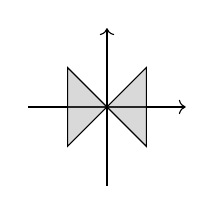
\begin{tikzpicture}
 \draw[->] (0,-1) -- (0,1);
 \draw[->] (-1,0) -- (1,0);
 \draw[fill=gray, fill opacity=0.3] (0,0) -- (0.5,-0.5) -- (0.5,0.5) -- (0,0) -- (-0.5,0.5) -- (-0.5,-0.5) -- cycle;
\end{tikzpicture}\]
\end{Example}

\begin{Definition}
 Let $R$ be a normed field and let $\mathbb{V}$ be a topological $R$-vector space. We say that $\mathbb{V}$ is \emph{locally convex} iff every $x\in \mathbb{V}$ admits a local basis consisting of disks at $x$.
 Since the topology of $\mathbb{V}$ is necessarily translation invariant,
 it is equivalent to only ask that $0$ has such a local basis.
\end{Definition}

\begin{Proposition}\label{prop:mainLCTVS}
 Let $\mathbb{V}$ be a locally convex topological $\R$-vector space (where $\R$ is endowed with its usual absolute value and the induced topology by it).
 Fix $x\in\mathbb{V}$, a neighbourhood $V\subseteq\mathbb{V}$ of $x$ and $f:V\to \R\cup\set{+\infty,-\infty}$.
 If $V$ is convex, $f$ is concave and lower bounded by a finite constant $K$, then $f$ is continuous at $x$ (w.r.t.\ the subspace topology on $V$).
\end{Proposition}
\begin{proof}
 Since $V$ is a neighbourhood of $x$, $x$ admits an open neighbourhood $U\subseteq V$, and by local convexity of $\mathbb{V}$ there is a (non necessary open) disk $D\subseteq U$ at $x$.
 Now fix $\eps\in(0,1)$ and $r,s\in \R$ with $0\leq r\leq\eps$, $s=1-r$.
 Fix also $w\in D$.
 By the convexity of $D$ we have $sx+rw\in D$, and thus the convexity of $f$ entails that:
 \[
  f(sx+rw)\geq s f(x) + r f(w) \geq s f(x) + r K = (1-r)f(x) + r K
 \]
that is,
 \[
  f(x)-f(sx+rw)\leq r (f(x)-K).
 \]
 Now remark that $x=\dfrac{1}{s+2r}(sx+rw)+\dfrac{r}{s+2r}(2x-w)$, where $\dfrac{1}{s+2r}+\dfrac{r}{s+2r}=1$, $\dfrac{1}{s+2r}<1$ and $2x-w\in D$ (because $D$ is a disk at $x$).
 Therefore by the convexity of $f$ we have:
 \[
  f(x)\geq \dfrac{1}{s+2r}f(sx+rw)+\dfrac{r}{s+2r}f(2x-w)\geq \dfrac{1}{s+2r}(f(sx+rw)+rK)
 \]
 that is,
 \[
  f(sx+rw)-f(x)\leq r(f(x)-K).
 \]
 We have thus shown that $\mid f(sx+rw)-f(x)\mid\leq r(f(x)-K)$ for all $w\in D$.
 Since this holds also for all $\eps\in(0,1)$, and due to the choice of $r,s$, the points of shape $sx+rw$ span $D$ when $w$ spans $D$ and $\eps$ spans $(0,1)$.
 That is, we have shown that $\mid f(w)-f(x)\mid\leq r(f(x)-K)$ for all $w\in W$.
 Since $f(x)-K\geq 0$ and $r\leq \eps$, we have that $\exists\lim\limits_{w\to x} f(w)=f(x)$.
\end{proof}

\begin{Corollary}\label{cor:cont}
 Let $f:({\R}_{> 0}^X,\supnorm{.}) \to (\overline\R_{\geq 0},\absv .)$ and $x\in {\R}_{> 0}^X$.
 If there is a convex neighbourhood $V\subseteq \overline{\R}_{> 0}^X$ of $x$ s.t.\ $f_{\big\mid V}$ is concave, then $f$ is continuous at $x$.
\end{Corollary}
\begin{proof}
 The $\R$-vector space $\R^X$ is topological w.r.t.\ the topology $\tau_\infty$ induced on it by the norm $\lVert .\lVert_\infty$, and it is clearly locally convex.
 Call $\tau^+_\infty$ the topology induced by $\supnorm{.}$ on ${\R}_{> 0}^X$.
 It is clear that it coincides with $\tau^+_\infty$.
 Since moreover ${\R}_{> 0}^X$ is open in $(\R^X,\tau_\infty)$, the neighbourhood $V$ of $x$ in $({\R}_{> 0}^X,\supnorm{.})$ is also a neighbourhood of $x$ in $(\R^X,\tau_\infty)$.
 We can therefore apply Proposition~\ref{prop:mainLCTVS} to $f_{\big\mid V}$ (which is lower bounded by $0$ by definition of $f$) and obtain that $f_{\big\mid V}$ is continuous at $x$ w.r.t.\ the subspace topology $\tau_V$ induced by $\tau_\infty$ on $V$.
 But since $V$ is contained in ${\R}_{> 0}^X$, the topology $\tau_V$ coincides with the subspace topology induced on $V$ by $\tau^+_\infty$.
 So $f$ is continuous at $x$ w.r.t.\ $\tau^+_\infty$.
\end{proof}

One may wonder if the same proof as above makes it possible to state the previous corollary replacing ${\R}_{> 0}^X$ with $\R_{\geq 0}^X$ (so, in particular, taking $x\in\R_{\geq 0}^X$).
This is not possible because in the proof we crucially use that $\R_{> 0}^X$ is open in $(\R^X,\tau_\infty)$, which is not the case of $\R_{\geq 0}^X$.
In fact, this allowed us to say that $V$ is a neighbourhood of $x$ in $(\R^X,\tau_\infty)$, and therefore to be able to apply Proposition~\ref{prop:mainLCTVS}.
Taking $\R_{\geq 0}^X$ instead, this is in general not true: we could have a neighbourhood of $x$ w.r.t.\ the subspace topology on $\R_{\geq 0}^X$ induced by $\tau_\infty$, which does not contain any open neighbourhood of $x$ w.r.t.\ $\tau_\infty$ (i.e. it is not a neighbourhood w.r.t.\ $\tau_\infty$).

\begin{Example}
 An example of a neighbourhood of $x$ w.r.t.\ the subspace topology on $\R_{\geq 0}^X$ induced by $\tau_\infty$, which is not a neighbourhood w.r.t.\ $\tau_\infty$.
 \[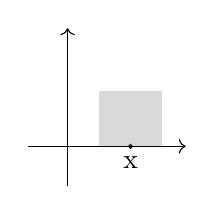
\begin{tikzpicture}
 \draw[->] (0,-0.5) -- (0,1.5);
 \draw[->] (-0.5,0) -- (1.5,0);
 \filldraw[black] (0.8,0) circle (0.7pt) node[anchor=north]{x};
 \fill[fill=gray, fill opacity=0.3] (0.4,0) -- (1.2,0) -- (1.2,0.7) -- (0.4,0.7) -- (0.4,0) -- cycle;
\end{tikzpicture}\]
\end{Example}


\begin{Corollary}\label{cor:tropCont}
 Tropical functions $f:({\R}_{\geq 0}^X,\supnorm .) \to (\overline\R_{\geq 0},\absv .)$ are continuous on ${\R}_{> 0}^X$.
\end{Corollary}
\begin{proof}
 We know that tropical functions are concave on all their domain.
 Therefore the result immediate follows by Corollary \ref{cor:cont}, since the topology induced by $\supnorm{.}$ on ${\R}_{> 0}^X$ coincides with the subspace topology induced by $({\R}_{\geq 0}^X,\supnorm .)$ on it.
\end{proof}

Due to the previous discussion about the impossibility of stating Corollary \ref{cor:cont} in the case where one of the coordinates of $x$ is $0$, the continuity of tropical functions on the hyperplanes $\mathcal H_a:=\set{x\in {\R}_{\geq 0}^X \mid x_a=0}$, for $a\in X$, must be treated separately.
Similarly, the continuity at points with infinite coordinates must be treated separately as well.

Discussione sui coni ? (Vedi altra pagina)

\newpage

\begin{Definition}
 An \emph{$\overline{\R}_{\geq 0}$-cone} is a commutative $\overline{\R}_{\geq 0}$-semimodule with cancellative addition\footnote{I.e.: $x+y=x+y' \Rightarrow y=y'$.}.
\end{Definition}

In [Selinger] cones are required to also have ``strict addition'', meaning that $x+y=0 \Rightarrow x=y=0$.
We do not add this requirement since it will automatic hold when considering normed cones.

\begin{Remark}
 The addition of a cone $P$ (which forms a commutative monoid) turns $P$ into a poset by setting:
 \[
  x \leq y \textit{ iff } y=x+z \textit{, for some }z\in P.
 \]
 By the cancellative property, when such $z$ exists it is unique, and we denote it by $y-x$.
 Such order is called the \emph{cone-order} on $P$.
\end{Remark}

\begin{Definition}
 A \emph{normed $\overline{\R}_{\geq 0}$-cone} is the data of a $\overline{\R}_{\geq 0}$-cone together with a $\leq$-monotone\footnote{I.e.: $x\leq y \Rightarrow \norm{x}\leq \norm y$. Remark that requiring this property (for all $x,y$) is equivalent to requiring that $\norm{x}\leq \norm{x+y}$ for all $x,y$.} norm\footnote{A \emph{norm} on a $\overline{\R}_{\geq 0}$-abstract cone $P$ is a map $\norm{.}:P\to \overline{\R}$ satisfying the usual axioms of norms:
 $\norm x \geq 0$, $\norm x = 0 \Rightarrow x=0$, $\norm{rx}=r\norm x$ and $\norm{x+y}\leq \norm x + \norm y$.} on it.
\end{Definition}

In [Ehrhard-Pagani-Tasson, Crubillie] a normed $\overline{\R}_{\geq 0}$-cone is simply called a cone.

Remark that in a normed $\overline{\R}_{\geq 0}$-cone, by monotonicity of the norm, we have: $\norm{x+y}=0 \Rightarrow x=y=0$.
Therefore, as already mentioned, in a normed cone we have: 
$x+y=0 \Rightarrow \norm{x+y}=0 \Rightarrow x=y=0$, that is, addition is strict.

\begin{Example}
 $\overline{\R}_{\geq 0}^X$ is a normed cone with the norm $\supnorm{x}:=\sup\limits_{a\in X} x_a\in \overline{\R}_{\geq 0}$.
\end{Example}

\begin{Notation}
 We call $\overline{\mathscr{B}}^{\norm{.}}_1(P)$ the closed unit ball $\set{x\in\overline{\R}_{\geq 0}\mid \norm{x}\leq 1}$ of a normed $\overline{\R}_{\geq 0}$-cone $P$.
 We will also simply call it $\overline{\mathscr B}$ when the other informations are clear from the context.
 Similarly, $\mathscr B$ denotes the open unit ball.
\end{Notation}

\begin{Remark}
 The cone-order on $\overline{\R}_{\geq 0}^X$ is the pointwise usual order on $\overline{\R}_{\geq 0}$.
 
 Remark also that tropical functions have no reason to be linear nor sublinear.
\end{Remark}

\begin{Remark}\label{rmk:tropMonot}
 Tropical functions are monotone w.r.t.\ to the cone order on its domain and codomain.
 This is clear, using the definition of tropical functions, because $\mu x\leq \mu y$ if $x\leq y$.
\end{Remark}

\begin{Remark}
 The image $fD$ of a directed subset $D$ of a poset $P$ under a monotone function $f:P\to P'$ is always directed.
 This is clear because for all $x,y\in P$, we have $f(x)\leq f(z)\geq f(y)$, where $z\in D$ is s.t.\ $x\leq z\geq y$ and it exists in $D$ since $D$ is directed.
 \end{Remark}

\begin{Remark}
 The cone-order on $\overline{\R}_{\geq 0}^X$ makes it into a dcpo with least element $0$.
\end{Remark}

\begin{Lemma}\label{lm:sup=sup}
 Let $P$ be a poset and $X, I$ sets. Fix the pointwise order on $P^X$.
 \begin{enumerate}
  \item Let $x^i\in P^X$ for $i\in I$.
  If $\bigvee\limits_{i\in I} x^i$ exists $P^X$, then $\bigvee\limits_{i\in I} x^i_a$ exists in $P$ for all $a\in X$, and we have: \[\bigvee\limits_{i\in I} x^i_a=\left(\bigvee\limits_{i\in I} x^i\right)_a.\]
 \item Let $x^i_a\in P$ for $i\in I,a\in X$.
  If $\bigvee\limits_{i\in I} x^i_a$ exists $P$ for all $a\in X$, then $\bigvee\limits_{i\in I} x^i$ exists in $P^X$, and we have: \[\left(\bigvee\limits_{i\in I} x^i\right)_a=\bigvee\limits_{i\in I} x^i_a.\]
 \end{enumerate}
\end{Lemma}
\begin{proof}
 (1). Fix $a\in X$. Let us show that $\left(\bigvee\limits_{i\in I} x^i\right)_a$ is indeed the sup of $\set{x^i_a\mid i\in I}$.
 It is an upper bound because $\bigvee\limits_{i\in I} x^i\geq x^i$.
 Now let $d\in P$ be an upper bound of $\set{x^i_a\mid i\in I}$. In order to show that $d\geq \left(\bigvee\limits_{i\in I} x^i\right)_a$, let us consider $h\in P^X$ defined by $h_c:=\left(\bigvee\limits_{i\in I} x^i\right)_c$ if $c\neq a$ and $h_a:=d$.
 By construction $h$ is an upper bound of $\set{x^i\mid i\in I}$.
 So, by definition of sup, $h\geq \bigvee\limits_{i\in I} x^i$.
 Hence $d=h_a\geq\left(\bigvee\limits_{i\in I} x^i\right)_a$.
 
 (2). Analogue.
\end{proof}

A \emph{directed net} in a poset $P$ with indices in a set $I$ is a function $s:I\to P$, denoted by $(s_i)_{i\in I}$, s.t.\ its image is directed.
We say that a directed net in $P$ \emph{admits a sup} iff its image admits a sup in $P$.
We say that a directed net $s$ in a normed cone is \emph{bounded} iff the set $\set{\norm{s_i}\,\mid i\in I}$ is bounded in $\R_{\geq 0}$.
In the study of dcpo's the role played by sequences in usual topology is often played by directed nets.

\begin{Remark}\label{rmk:trivial}
 Monotone functions between posets transport directed nets to directed nets\footnote{We simply mean that if $(s_i)_i$ is a directed net in the domain, then $(f(s_i))_i$ is a directed net in the codomain.}.
\end{Remark}

\begin{Definition}
 A function $f:P\to P'$ between posets is \emph{Scott-continuous} iff for all directed net $(s_i)_i$ in $P$ admitting a sup, we have $\exists \bigvee\limits_i f(s_i) = f(\bigvee\limits_i s_i)$ in $P'$. 
\end{Definition}

As it is well known, the order theoretic notion of Scott-continuity coincides with the topological continuity w.r.t.\ to the \emph{Scott-topology} on $P$, whose opens are exactly the upward closed $O\subseteq P$ s.t.\ for all directed $D\subseteq P$ with $\bigvee D\in O$, one has $D\cap O\neq\emptyset$.

\begin{Proposition}\label{prop:infsup}
 Let $P$ be a normed $\overline{\R}_{\geq 0}$-cone s.t.\ every bounded directed net in $P$ admits a sup.
 Let $(v_i)_{i\in I}$ be a directed net in $P$ with an upper bound $v\in P$.
 Then $\exists\bigvee\limits_{i\in I} v_i \in P$ and, if $\inf\limits_{i\in I} \norm{v-v_i} =0$, one has: $\bigvee\limits_{i\in I} v_i = v$.
\end{Proposition}
\begin{proof}
 Remark that $v-v_i$ exists in $P$ by hypothesis and so does $\bigvee\limits_{i\in I} v_i$, thanks to the monotonicity of the norm.
 Now, since $v\geq v_i$ for all $i$, we have that $v\geq \bigvee\limits_{i\in I} v_i$, and so $v-\bigvee\limits_{i\in I} v_i$ exists in $P$.
 Fix $i\in I$.
 Since $v_i\leq \bigvee\limits_{i\in I} v_i$, then $v-\bigvee\limits_{i\in I} v_i\leq v-v_i$ and, by monotonicity of the norm, $\norm{v-\bigvee\limits_{i\in I} v_i}\leq \norm{v-v_i}$.
 Since this holds for all $i\in I$, we have:
 $0\leq \norm{v-\bigvee\limits_{i\in I} v_i}\leq \inf\limits_{i\in I} \norm{v-v_i}=0$, where the last equality holds by hypothesis.
 Thus $\norm{v-\bigvee\limits_{i\in I} v_i}=0$, i.e.\ $v=\bigvee\limits_{i\in I} v_i$.
\end{proof}

\begin{Definition}
 A normed $\overline{\R}_{\geq 0}$-cone $P$ is \emph{Scott-complete} iff its norm is Scott-continuous (where the codomain $\overline\R_{\geq 0}$ is endowed with its usual order) and every bounded directed net in $P$ admits a sup.
 This is equivalent to asking that its closed unit ball is a dcpo.
\end{Definition}

\begin{Proposition}
 The normed cone $\overline{\R}_{\geq 0}^X$ is Scott-complete.
\end{Proposition}
\begin{proof}
 $\overline{\R}_{\geq 0}^X$ being a dcpo, all the existences of sup's that we should check do automatically hold, so we only have to show that $\bigvee$ and $\supnorm{.}$ commute:
 $\supnorm{\bigvee\limits_i x_i}=
 \sup\limits_a\, \sup\limits_i\, (x_i)_a =
 \sup\limits_i\, \sup\limits_a\, (x_i)_a =
 \bigvee\limits_i \supnorm{x_i}$.
\end{proof}

%Let us set $\infty_b$ to be the hyper-semi-plane $\set{y\in\overline{\R}^Y_{\geq 0}\mid y_b=+\infty}$ and $\set{f<<+\infty}:=\bigcup\limits_{b\in Y} f^{-1}\infty_b$.

%\begin{Remark}\label{rmk:R-f<<oo}
%Let $f:\overline{\R}^X_{\geq 0}\to\overline{\R}^Y_{\geq 0}$ be tropical.
%Then, $\R^X_{> 0}-\set{f<<+\infty}$ is a dcpo (w.r.t.\ the usual order, that is, its cone order).
%In order to see this, it is enough to show that, for any $b\in Y$ and for any directed net $(x^i)_i$ in $\R^X_{> 0}$ s.t.\ $f(x^i)_b<+\infty$ for all $i$, we have $f(\bigvee\limits_i x^i)_b<+\infty$ (where the sup is taken in $\R^X_{> 0}$).
%Such property holds because otherwise it is easy to see that $f$ would be discontinuous at the point $\bigvee\limits_i x^i\in\R^X_{> 0}$ w.r.t.\ the topology\footnote{Remark that this argument would not be possible using Scott-continuity instead. Indeed, it could well be that $f(\bigvee\limits_i x^i)_b=\bigvee\limits_i f(x^i)_b=+\infty$ while $f(x^i)_b<+\infty$ for all $i$.} induced by $\supnorm{.}$.
%This contradicts Corollary \ref{cor:tropCont}.
%\end{Remark}

\begin{Proposition}
 All tropical functions $f:\overline{\R}^X_{\geq 0}\to\overline{\R}^Y_{\geq 0}$ are Scott-continuous on $\R^X_{> 0}$ w.r.t.\ the cone-orders on its domain and codomain.
\end{Proposition}
\begin{proof}
 Let $(x_i)_i$ a directed net in $\R^X_{> 0}$ s.t.\ $\bigvee\limits_i x^i$ exists in $\R^X_{> 0}$.
 Then $\inf\limits_i \supnorm{\bigvee\limits_i x^i - x^i} =0$, where $\bigvee\limits_i x^i - x^i$ exists because $\bigvee\limits_i x^i \geq x^i$ for all $i$.
 Since $f$ is $\supnorm{.}$-continuous on $\R^X_{> 0}$ (Corollary \ref{cor:tropCont}), then $\inf\limits_i \supnorm{f(\bigvee\limits_i x^i) - f(x^i)} =0$, where $f(\bigvee\limits_i x^i) - f(x^i)$ exists because $f(\bigvee\limits_i x^i) \geq f(x^i)$ for all $i$ being $f$ monotone (Remark \ref{rmk:tropMonot}).
 We can therefore apply Proposition \ref{prop:infsup} to the directed net $(f(x^i))_i$ in $\overline{\R}^Y_{\geq 0}$, obtaining that $\bigvee\limits_i f(x^i)$ exists in $\overline{\R}^Y_{\geq 0}$ and it coincides with $f(\bigvee\limits_i x^i)$.
\end{proof}

%\begin{Remark}
%By looking at the definition of tropical functions, for $f$ tropical we have that: if $x,x'\in\R^X_{> 0}-\set{f<<+\infty}$ and $r\in\R_{> 0}$, then $x+x',rx\in\R^X_{> 0}-\set{f<<+\infty}$.
%That is, $\R^X_{> 0}-\set{f<<+\infty}$ is a $\R_{>0}$-cone.
%It is clearly still Scott-complete.
%\end{Remark}

\begin{Definition}
 Let $P$ be a dcpo.
 We define a relation by: $x<<y$ iff for all directed $D\subseteq P$, if $y\leq \bigvee D$, then $x\leq d$, for some $d\in D$.
 Call $\twoheaddownarrow y:=\set{x\in P\mid x<<y}$.
 A dcpo $P$ is \emph{Scott-continuous} iff $\twoheaddownarrow x$ is directed and $x=\bigvee\twoheaddownarrow x$ for all $x\in P$.
\end{Definition}

\begin{Remark}
 In any dcpo we have: $\twoheaddownarrow x \subseteq \downarrow x$.
 This immediately follows by considering the directed set $\set{x}$.
\end{Remark}

\begin{Lemma}\label{lm:<<dir}
 In $\overline{\R}_{\geq 0}^X$, every set $\twoheaddownarrow x$ is directed.
\end{Lemma}
\begin{proof}
 It is immediate that $0\in\twoheaddownarrow x$, so it is non-empty.
 Now let $y,y' << x$.
 Since we are in $\overline{\R}_{\geq 0}^X$, there is $y\vee y'\in\overline{\R}_{\geq 0}^X$.
 So we only have to show that $y\vee y'<<x$.
 For that, let $D$ be a directed set in $\overline{\R}_{\geq 0}^X$ s.t.\ $x\leq\bigvee D$.
 Since $y,y' << x$ we find $d,d'\in D$ s.t.\ $y\leq d$, $y'\leq d'$.
 Since $D$ is directed, there is $\hat d\in D$ s.t.\ $y\leq d\leq \hat d\geq d'\geq y'$.
 But then, by definition of sup, it must be $\hat d\geq y\vee y'$ and we are done.
\end{proof}

\begin{Remark}
 The following is a known property (that we will not use):
 let $P$ be a complete normed cone which is a dcpo w.r.t.\ its cone-order. Then $P$ is Scott-continuous as a dcpo iff its closed unit ball is Scott-continuous as a dcpo.
\end{Remark}

\begin{Remark}\label{rmk:<<R}
 Consider $\overline{\R}_{\geq 0}$ with its usual order (which coincides with its cone-order).
 It is easily seen (and well known) that $y<<x$ iff either $y=0$ or $y<x$.
 This immediately implies that $\overline{\R}_{\geq 0}$ is Scott-continuous, since $x=\sup\limits_{y<x} y$.
\end{Remark}

\begin{Lemma}\label{lm:<<RX}
 Let $x,y\in \overline{\R}_{\geq 0}^X$ (considered as a dcpo with its cone order, which is the pointwise one). Fix $a\in X$.
 If $y_a<<x_a$ and $y_c=0$ for all $c\neq a$, then $y<<x$.
\end{Lemma}
\begin{proof}
 Towards a contradiction, assume that there is a directed set $D$ in $\overline{\R}_{\geq 0}^X$ with $x\leq\bigvee D$ and s.t.\ $y\not\leq d$ for all $d\in D$.
 Call $D_a:=\set{d_a\mid d\in D}$ and remark that it is directed, because $D$ is.
 Also, by Lemma \ref{lm:sup=sup}, $\bigvee D_a = \left(\bigvee D\right)_a$.
 Therefore from $y_a<<x_a\leq \bigvee D_a$ we obtain a $d\in D$ s.t.\ $y_a\leq d_a$.
 By the absurd hypothesis we have $y\not\leq d$, so there must be $c\in X$ s.t.\ $y_c\not\leq d_c$, i.e. (because real numbers are totally ordered) $y_c>d_c$.
 Therefore it must be $c\neq a$.
 But then we have $0=y_c>d_c\geq 0$, contradiction.
\end{proof}

\begin{Lemma}\label{lm:<<_a}
 In $\overline{\R}_{\geq 0}^X$ we have:
 if $y<<x$ then $y_a<< x_a$ for all $a\in X$.
\end{Lemma}
\begin{proof}
 Fix $a\in X$.
 Let $D$ directed set in $\overline{\R}_{\geq 0}$ s.t.\ $x_a\leq\bigvee D$.
 We look for a $d\in D$ s.t.\ $y_a\leq d$.
 For $d\in D$, let $x^{a,d}\in\overline{\R}_{\geq 0}^X$ defined by $x^{a,d}_c:=x_c$ if $c\neq a$ and $x^{a,d}_a:=d$.
 Let $D^x_a:=\set{x^{a,d}\mid d\in D}$.
 By Lemma \ref{lm:sup=sup} $D^x_a$ admits sup in $\overline{\R}_{\geq 0}^X$ and it is $(\bigvee D^x_a)_c=x_c$ if $c\neq a$ and $(\bigvee D^x_a)_a=\bigvee D$.
 Hence, $x\leq \bigvee D^x_a$.
 If we prove that $D^x_a$ is directed, we are done: indeed, since $y<<x$, there is $d\in D$ s.t.\ $y\leq x^{a,d}$ and thus, in particular, $y_a\leq x^{a,d}_a=d$.
 Let us finally prove that $D^x_a$ is directed: it is clearly non-empty, since $D$ is.
 Let now $d,d'\in D$.
 We want to show that there is $\hat d\in D$ s.t.\ $x^{a,d}\leq x^{a,\hat d}\geq x^{a,d'}$.
 But since $D$ is directed, there is $\hat d\in D$ s.t.\ $d\leq \hat d\geq d'$, and therefore $x^{a,d}_c=x_c= x^{a,\hat d}_c =x_c=x^{a,d'}_c$ for all $c\neq a$, and $x^{a,d}_a=d\leq \hat d=x^{a,\hat d}_a=\hat d \geq d'=x^{a,d'}_a$.
\end{proof}

\begin{Lemma}\label{rmk:sup_a=sup_a}
In $\overline{\R}_{\geq 0}^X$ we have:
$\bigvee\limits_{y<<x_a} y = \bigvee\limits_{y<<x} y_a$.
\end{Lemma}
\begin{proof}
 If we show that $\twoheaddownarrow x_a = \set{y_a\mid y\in\twoheaddownarrow x}$, then we are done because in the statement we are taking their sup's.
 The inclusion ($\supseteq$) immediately follows from Lemma \ref{lm:<<_a}. For ($\subseteq$), let $d<< x_a$.
 Then the $y\in \overline{\R}_{\geq 0}^X$ defined by $y_c:=0$ if $c\neq a$ and $y_a:=d$, is s.t.\ $y\in\twoheaddownarrow x$ by Lemma \ref{lm:<<RX}.
 Thus, $d\in \set{y_a\mid y\in\twoheaddownarrow x}$.
\end{proof}


\begin{Corollary}
 The dcpo $\overline{\R}_{\geq 0}^X$ is Scott-continuous.
\end{Corollary}
\begin{proof}
 The fact that $\twoheaddownarrow x$ is directed is given by Lemma \ref{lm:<<dir}. The fact that $x=\bigvee \twoheaddownarrow x$ is given by the following equalities:
 $x_a=\bigvee\limits_{y<<x_a} y = \bigvee\limits_{y<<x} y_a = \left(\bigvee\limits_{y<<x} y\right)_a=\left(\bigvee \twoheaddownarrow x\right)_a$.
 The first equality follows from Remark \ref{rmk:<<R}, the second one from Lemma \ref{rmk:sup_a=sup_a}, the third one from Lemma \ref{lm:sup=sup}.
\end{proof}



%\section{Bibliography}

\end{document}
